\section{}\label{section}

\subsection{}\label{section-1}

\begin{enumerate}
\def\labelenumi{\arabic{enumi}.}
\item
  \begin{center}\rule{0.5\linewidth}{0.5pt}\end{center}
\item
  \textbf{WebGLThree.js}WebGLThree.jsAPI
\item
  \begin{center}\rule{0.5\linewidth}{0.5pt}\end{center}
\item
  \begin{center}\rule{0.5\linewidth}{0.5pt}\end{center}
\item
  \begin{center}\rule{0.5\linewidth}{0.5pt}\end{center}
\item
  \begin{center}\rule{0.5\linewidth}{0.5pt}\end{center}
\end{enumerate}

\subsection{}\label{section-2}

WebGLThree.js

WebWebGLWebThree.js

\subsection{}\label{section-3}

!!! info ``\,''

\begin{verbatim}
### [ ](section06-01.md)
- - 
- - 

### [ WebGL](section06-02.md) 
- WebGL
- - 
- WebGL

### [ Three.js](section06-03.md)
- Three.js
- - 
- ### [ ](section06-04.md)
- - 
- - LOD

### [ ](section06-05.md)
- - 
- - 

### [ ](section06-06.md)
- - 
- - 
\end{verbatim}

\subsection{}\label{section-4}

\begin{longtable}[]{@{}lll@{}}
\toprule\noalign{}
\endhead
\bottomrule\noalign{}
\endlastfoot
API & WebGLOpenGL ES & \\
& Three.jsBabylon.js & \\
& & \\
& & \\
& LOD & \\
\end{longtable}

\subsection{}\label{section-5}

!!! tip ``\,''

\begin{verbatim}
=== ""
    - **Three.js**JavaScript 3D
    - **Babylon.js**Web 3D  
    - **A-Frame**HTMLVR
    - **PlayCanvas**3D
    
=== ""
    - **Blender**
    - **3ds Max**
    - **Maya**
    - **SketchUp**
    
=== ""
    - **Visual Studio Code**
    - **WebStorm**JavaScript IDE
    - **Chrome DevTools**
    - **Webpack**
\end{verbatim}

\subsection{}\label{section-6}

!!! note ``\,''

\begin{verbatim}
- **WebGL**Web Graphics LibraryOpenGL ESWeb
- ****GPU
- ****
- ****
- ****
- ****
\end{verbatim}

\subsection{}\label{section-7}

!!! example ``\,''

\begin{verbatim}
1. ****Three.js
2. ****
3. ****
4. ****
5. ****
\end{verbatim}

\subsection{}\label{section-8}

!!! note ``\,''

\begin{verbatim}
- **WebGPU**WebAPIGPU
- ****Web
- **WebAssembly**WASM
- ****GPU
- ****Web
\end{verbatim}

\subsection{}\label{section-9}

{[}1{]} Khronos Group. WebGL 2.0 Specification{[}S{]}. Khronos Group
Inc, 2017.

{[}2{]} Dirksen J. Learn Three.js: Programming 3D animations and
visualizations for the web with HTML5 and WebGL{[}M{]}. 4th
ed.~Birmingham: Packt Publishing, 2023.

{[}3{]} Angel E, Shreiner D. Interactive Computer Graphics: A Top-Down
Approach with WebGL{[}M{]}. 7th ed.~Boston: Pearson, 2014.

{[}4{]} Akenine-Möller T, Haines E, Hoffman N. Real-Time
Rendering{[}M{]}. 4th ed.~Boca Raton: CRC Press, 2018.

{[}5{]} Marschner S, Shirley P. Fundamentals of Computer
Graphics{[}M{]}. 5th ed.~Boca Raton: CRC Press, 2021.

\subsection{}\label{section-10}

\subsubsection{}\label{section-11}

\begin{enumerate}
\def\labelenumi{\arabic{enumi}.}
\tightlist
\item
  WebGL
\item
  Three.js
\item
\end{enumerate}

\subsubsection{}\label{section-12}

\begin{enumerate}
\def\labelenumi{\arabic{enumi}.}
\tightlist
\item
\item
\item
\end{enumerate}

\subsubsection{}\label{section-13}

\begin{enumerate}
\def\labelenumi{\arabic{enumi}.}
\tightlist
\item
\item
  Web
\end{enumerate}

\subsection{}\label{section-14}

WebGLThree.js

\subsection{}\label{section-15}

``\,''

``\,''\,``\,''\,``\,''\,``\,''

\subsection{}\label{section-16}

\subsubsection{}\label{section-17}

\begin{enumerate}
\def\labelenumi{\arabic{enumi}.}
\tightlist
\item
\item
\item
\end{enumerate}

\subsubsection{}\label{section-18}

\begin{enumerate}
\def\labelenumi{\arabic{enumi}.}
\tightlist
\item
\item
\item
\end{enumerate}

\subsubsection{}\label{section-19}

\begin{enumerate}
\def\labelenumi{\arabic{enumi}.}
\tightlist
\item
\item
\end{enumerate}

\subsection{}\label{section-20}

\subsection{6.1}\label{section-21}

``\,''

GISBIM``\,''\,``\,''\,``\,''

\subsubsection{6.1.1}\label{section-22}

DEM, Digital Elevation ModelDSM, Digital Surface ModelTIN

BIM

L-system

GISBIM

\paragraph{6.1.1.1}\label{section-23}

Digital Elevation ModelDEM)Digital Terrain ModelDTMDigital Terrain Model
DTMDTM GISXYZ``\,''DSMDTM ``\,''

\[
K_p = f_k(u_p,v_p)(k=1,2,3,\cdots,m;p=1,2,3,\cdots,n)
\] (6.1.1)

\emph{\(K_p\)}\(p\)\emph{,}\(k\)\emph{\(u_p,v_p\)}p\textbf{m}m\emph{1)}n\textbf{n}n

(6.1.1)\emph{m}=1(\(u_p,v_p\))(6.1.1)DEM)DEMDTMDEMDTM

DEM\emph{D}

\[
V_=(X_i,Y_i,Z_i)(i=1,2,3,\cdots,n)
\] (6.1.2)

\(X_i,Y_i\), \(Z_i\)(\(X_i,Y_i\)),,DEM\(|Z_i,i=1,2,3,\cdots,n|\)

DEM

1

2,DEM,DEM

3,,DEM,,,::,1mDEM10m100mDEM;

1

DEMs(Local),

DEMs(Global),,

DEMs(Regional)

2

DEMs(Discontinuous):,,

DEMs(Continuous):DEMs,,,,DEMs

DEMs(Smooth):DEMs,:,

BIMGIS

CADRevit LiDAR BIM RevitTekla SketchUp3ds MaxGIS ArcGISCesium

/VR/AR

DEM

LiDAR

CesiumUnity 3DUnreal EngineMIKEHEC-RASOpenFOAM

L-systemsL

AI

\paragraph{6.1.1.2}\label{section-24}

MaterialTextureTexture MapMaterialTextureTexture Map3D

①3D②3D③④Photoshop⑤3D⑥⑦⑧UV3DUVUV2D3D⑨

\paragraph{6.1.1.3}\label{section-25}

1

\(I_e=K_aI_a\)\(I_a\)\(K_a\)\(I_e\)

2

\(I_d=I_pK_d cos \theta\)\(I_p\)\(K_d\)\(\theta\)

3

4

5

RGBRGB

6

7

GPU

123(Ray Tracing)(Radiosity)

\paragraph{6.1.1.4}\label{section-26}

ShaderUVSPHFLIPCaustics

GPUShader``\,''

Volumetric FogExponential Fog

Volumetric CloudsPerlin NoiseWorley Noise

UnityUnrealCesiumShaderGPULODAI

\paragraph{6.1.1.5}\label{section-27}

``\,''\,``\,''\,``\,''

UIUI``\,''\,``\,''

Ray Casting

``\,''\,``\,''\,``\,''\,``\,''\,``\,''

VR/AR``\,''Natural Interaction

``\,''\,``\,''VueReactUICesiumThree.jsUnity``--''AI

``\,''\,``\,''

\subsubsection{6.1.2}\label{section-28}

\paragraph{6.1.2.1 (LiDAR)}\label{lidar}

6.1.1(a)6.1.1(b)

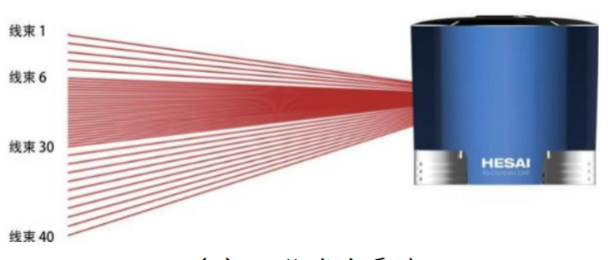
\includegraphics{images/ch6_image19.png}
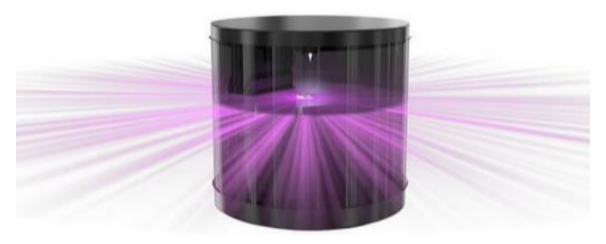
\includegraphics{images/ch6_image20.png}

\begin{enumerate}
\def\labelenumi{(\alph{enumi})}
\tightlist
\item
  \begin{enumerate}
  \def\labelenumii{(\alph{enumii})}
    \tightlist
  \item
  \end{enumerate}
\end{enumerate}

\textbf{6.1.1 }

6.1.2 CCD CCD*β**f* CCD \emph{d}3\%

\begin{figure}
\centering
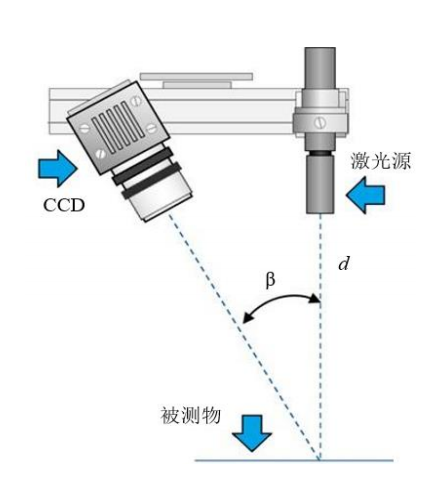
\includegraphics{images/ch6_image21.png}
\caption{06.3}
\end{figure}

\textbf{6.1.2 }

Time Of Flight6.1.3 \emph{t}1\emph{t}2(6.1.3)

\[
d=\Delta \times \frac{c}{2} (6.1.3)
\] \$c\$300000km/s

\textbf{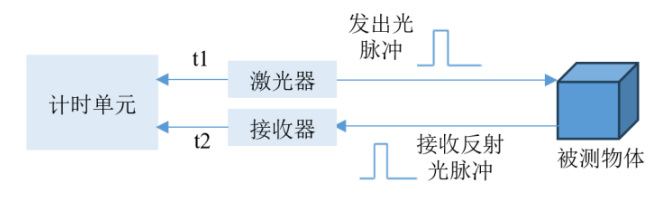
\includegraphics{images/ch6_image25.png}}

\textbf{6.1.3 TOF}

TOF TOF TOF

\paragraph{6.1.2.2}\label{section-29}

1

UAV;;;6.1.46.1.1

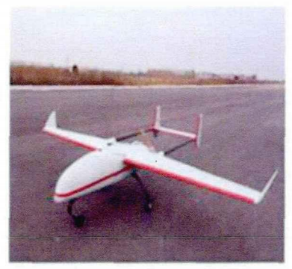
\includegraphics{images/ch6_image26.png}
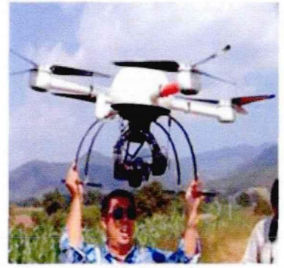
\includegraphics{images/ch6_image27.png}
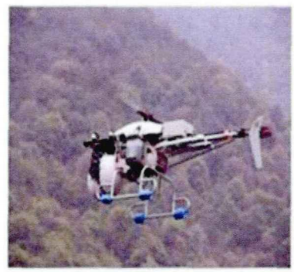
\includegraphics{images/ch6_image28.png}
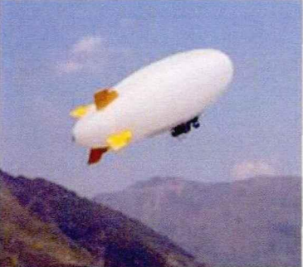
\includegraphics{images/ch6_image29.png}

\begin{enumerate}
\def\labelenumi{(\alph{enumi})}
\tightlist
\item
  \begin{enumerate}
  \def\labelenumii{(\alph{enumii})}
    \tightlist
  \item
    \begin{enumerate}
    \def\labelenumiii{(\alph{enumiii})}
        \tightlist
    \item
      \begin{enumerate}
      \def\labelenumiv{(\alph{enumiv})}
            \tightlist
      \item
      \end{enumerate}
    \end{enumerate}
  \end{enumerate}
\end{enumerate}

\textbf{6.1.4 }

\textbf{6.1.1 }

\textbf{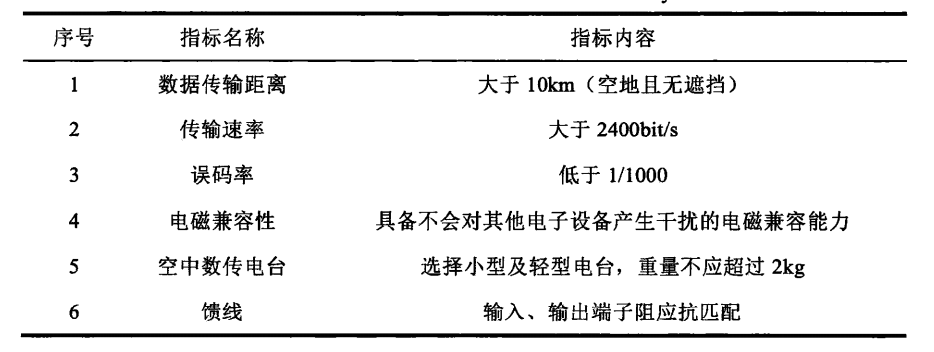
\includegraphics{images/ch6_image33.png}}

\textbf{6.1.2 }

\textbf{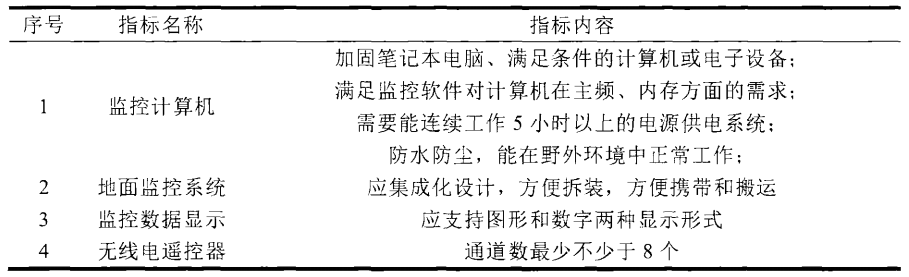
\includegraphics{images/ch6_image34.png}}

2

,``\,''\,``\,''\,``\,''6.1.5(1)1002kg(2):±3°(3)±20+5°

\begin{figure}
\centering
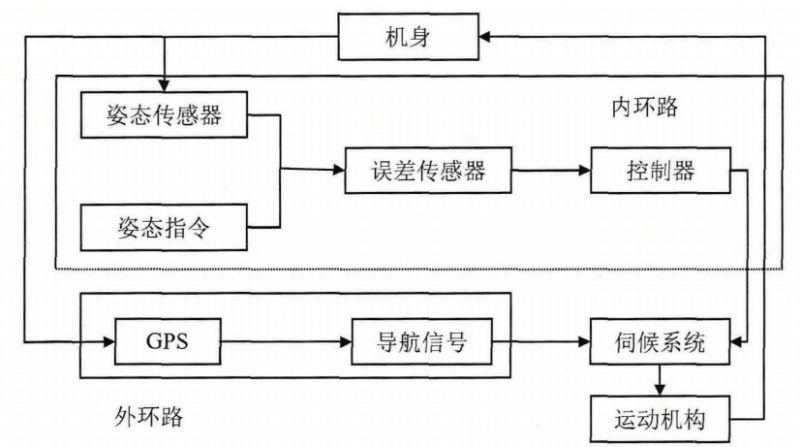
\includegraphics{images/ch6_image32.png}
\caption{06.11}
\end{figure}

\textbf{6.1.5 }

1

CCDCCD

2

;6.1.3

\textbf{6.1.3 }

\begin{figure}
\centering
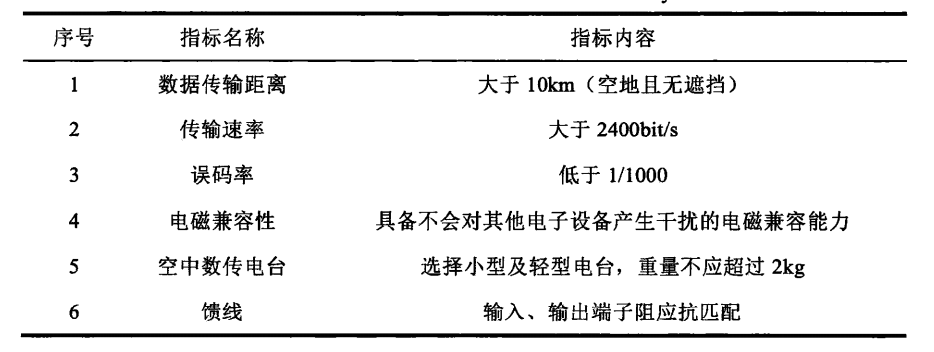
\includegraphics{images/ch6_image33.png}
\caption{06.12}
\end{figure}

3

6.1.4

\textbf{6.1.4 }

\begin{figure}
\centering
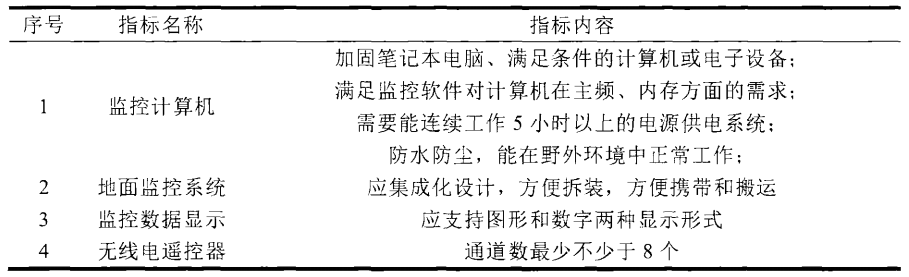
\includegraphics{images/ch6_image34.png}
\caption{06.13}
\end{figure}

::

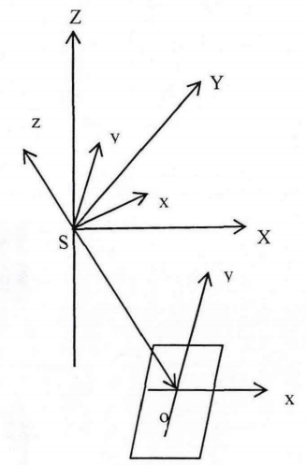
\includegraphics{images/ch6_image35.png}
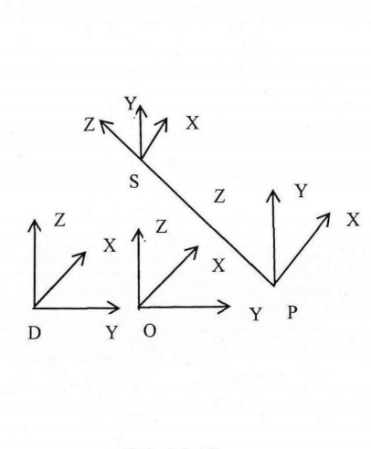
\includegraphics{images/ch6_image36.png}

\begin{enumerate}
\def\labelenumi{(\alph{enumi})}
\tightlist
\item
  \begin{enumerate}
  \def\labelenumii{(\alph{enumii})}
    \tightlist
  \item
  \end{enumerate}
\end{enumerate}

\textbf{6.1.6 }

①xy0-xy②2.7S-xz③S-XYZ

①S-XYZZPP-XpYpZpP②,-3°6°O-XtYtZt③6.1.6D-XtpYtpZtp

Sff;Ox0, y06.1.7

\begin{figure}
\centering
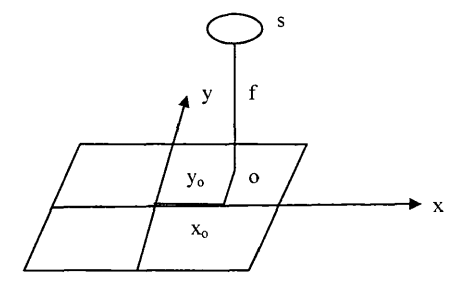
\includegraphics{images/ch6_image37.png}
\caption{06.16}
\end{figure}

\textbf{6.1.7 }

O\((x_0,y_0)\)\((x,y,f)\)

\[
\left\{ {\begin{array}{*{20}{c}}
{x = x' - {x_0}}\\
{y = y' - {y_0}}
\end{array}} \right.
\] (6.1.4)

1:2000

①53\%60\%\textsubscript{65\%15\%30\%}40\% 8\%``\,''65\%45\%②15
12°8°10\%8°15°,10°10\%215°30°20°315°10\%③\emph{d}3\% 30m50m
5\%④50\%30\%12\%⑤

\paragraph{6.1.2.3}\label{section-30}

GNSS

XYZDEM

GIS

GNSSRTKReal-Time KinematicGNSS

\paragraph{6.1.2.4}\label{section-31}

DEMDSMSAR

SVMRFCNN

MODISLandsatWorldView

\paragraph{6.1.2.5 CAD/BIM}\label{cadbim}

CAD

CAD Teigha

\begin{figure}
\centering
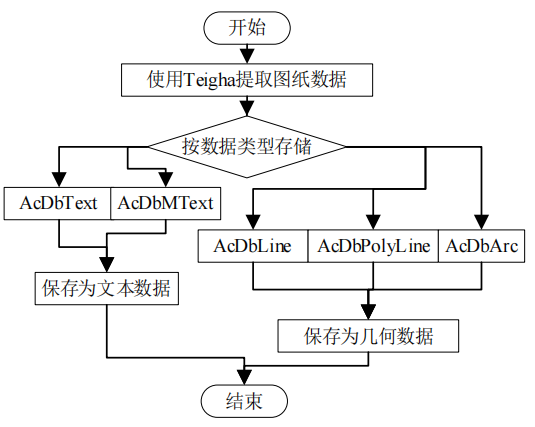
\includegraphics{images/ch6_image41.png}
\caption{06.17}
\end{figure}

\textbf{6.1.8 }

1

TeihgaCADBlockTable GetRXClass() Name
AcDbCircleAcDbArcAcDbPolyLineAcDbLine Teigha.DatabaseServices
CircleArcPolylineLine Layer Revit LineArcCirclePolyline
Autodesk.Revit.DBCurveLineArcCADGeometryModelTeighaLine ArcRevit Curve
TeighaCircleRevitArcTeighaPolylineXYZCadPolylinePointsLayerNameCadTextList
CADGeometryModelListCADGeometryModels

2

CAD RevitTeihgaCAD BlockTable
GetRXClass()NameAcDbTextAcDbMTextTeigha.DatabaseServicesTextMTextLayerCAD
Text Model List CADTextModel ListCADTextModels

3

CAD ``R''``r''``φ'' CAD

\begin{enumerate}
\def\labelenumi{(\arabic{enumi})}
\item
  CAD
\item
\item
\item
\item
\item
\item
\end{enumerate}

\begin{figure}
\centering
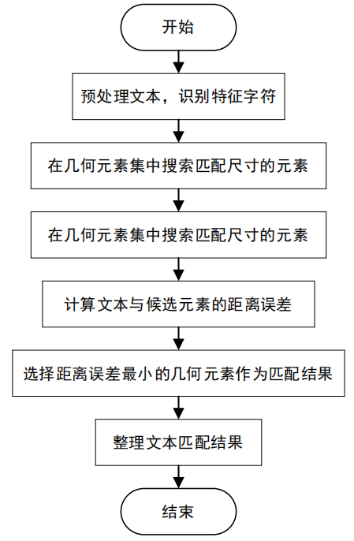
\includegraphics{images/ch6_image42.png}
\caption{06.18}
\end{figure}

\textbf{6.1.9 }

BIM

BIM CADCAD CADCAD Auto Desk AutoCAD Revit BIMCADBIM6.1.5

\textbf{6.1.5 BIMCAD}

\begin{figure}
\centering
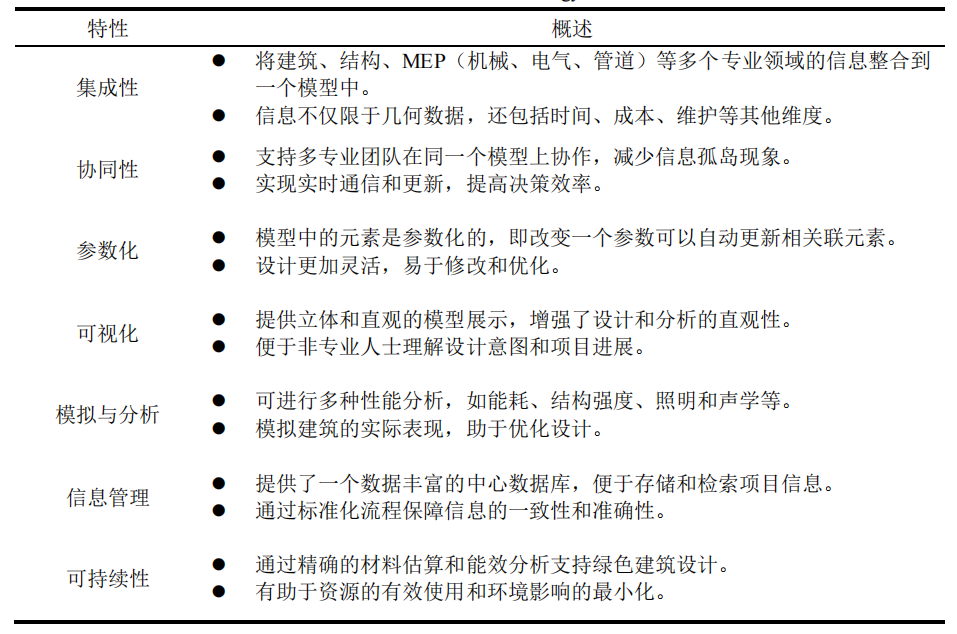
\includegraphics{images/ch6_image44.png}
\caption{06.19}
\end{figure}

BIMCADBIMBIM BIMBIMBIM CAD

BIMBIMBIMBIM6.1.6

\textbf{6.1.6 BIM}

\begin{figure}
\centering
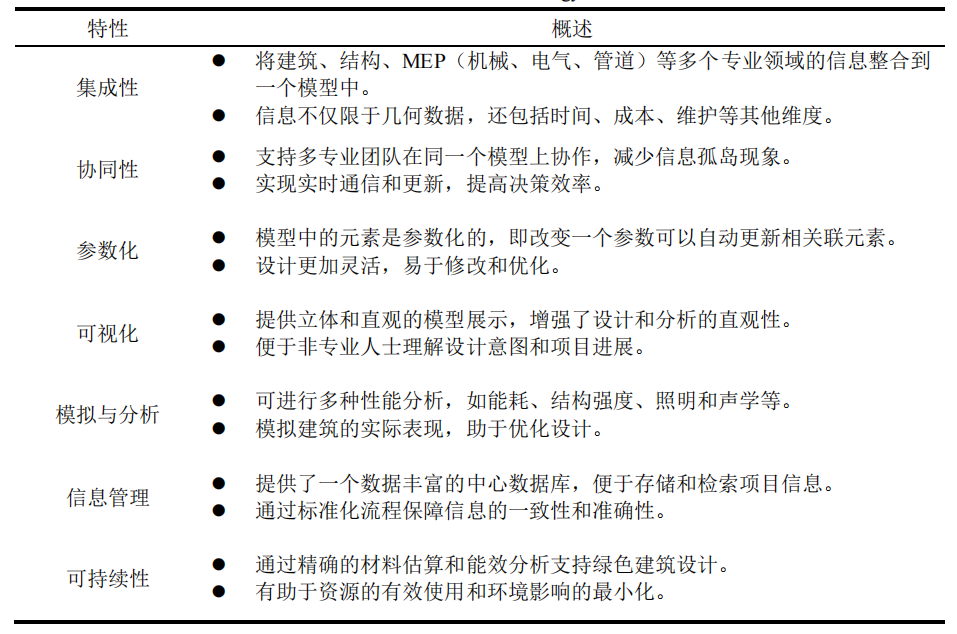
\includegraphics{images/ch6_image44.png}
\caption{06.20}
\end{figure}

BIMCADBIMBIMBIM

\subsubsection{6.1.3}\label{section-32}

\paragraph{6.1.3.1}\label{section-33}

``\,''

DEMHeightmapThree.js WebGL highmap

\begin{verbatim}
// Three.js

function createTerrainFromHeightmap(heightmapData, width, height, widthSegments, heightSegments) {

const geometry = new THREE.PlaneGeometry(

width, height, widthSegments, heightSegments

);

// 

const vertices = geometry.attributes.position.array;

for (let i = 0; i < vertices.length; i += 3) {

const x = Math.floor((i / 3) % (widthSegments + 1));

const y = Math.floor((i / 3) / (widthSegments + 1));

// 

const heightIndex = y \* width + x;

vertices[i + 2] = heightmapData[heightIndex] \* verticalScale;

}

geometry.computeVertexNormals();

// 

const material = new THREE.MeshPhongMaterial({

map: textureLoader.load('terrain\_texture.jpg'),

side: THREE.DoubleSide

});

return new THREE.Mesh(geometry, material);

}
```xml
heightmapData Z 

GIS Three.js  PlaneGeometry  Z  widthSegments  heightSegments computeVertexNormals()  terrain\_texture.jpg

LOD(Level of Detail)

LODLevel of DetailLOD

LODGPUThree.jsTHREE.LODLODLODThree.js

```javascript
// Three.jsLOD

function createLODTerrain(terrainData) {

const lod = new THREE.LOD();

// 

const highDetailGeometry = new THREE.PlaneGeometry(1000, 1000, 255, 255);

applyHeightmap(highDetailGeometry, terrainData, 1.0);

const highDetailMesh = new THREE.Mesh(

highDetailGeometry,

new THREE.MeshStandardMaterial({ map: highResTexture })

);

lod.addLevel(highDetailMesh, 0);

// 

const mediumDetailGeometry = new THREE.PlaneGeometry(1000, 1000, 127, 127);

applyHeightmap(mediumDetailGeometry, terrainData, 0.95);

const mediumDetailMesh = new THREE.Mesh(

mediumDetailGeometry,

new THREE.MeshStandardMaterial({ map: medResTexture })

);

lod.addLevel(mediumDetailMesh, 500);

// 

const lowDetailGeometry = new THREE.PlaneGeometry(1000, 1000, 63, 63);

applyHeightmap(lowDetailGeometry, terrainData, 0.9);

const lowDetailMesh = new THREE.Mesh(

lowDetailGeometry,

new THREE.MeshStandardMaterial({ map: lowResTexture })

);

lod.addLevel(lowDetailMesh, 1500);

return lod;

}

```javascript
 PlaneGeometry  255x255, 127x127, 63x63applyHeightmap Z1.00.950.9LOD lod.addLevel(mesh, distance) LODThree.js  highResTexturemedResTexturelowResTexture

LOD

1GPU

2

3LODVR

#### 6.1.3.2 

OpenGL6.1.10

**![06.21](images/ch6_image45.png)**

**6.1.10 OpenGL**

OpenGLRGBA46.1.11

![06.22](images/ch6_image46.png)

**6.1.11 **

Global IlluminationLocal LightingAmbient Occlusion, AO

1Local Lighting

Point LightDirectional LightSpot LightArea Light Phong  Blinn-Phong AmbientDiffuseSpecular

2Global Illumination, GI

Ray TracingPath TracingRadiosityPhoton Mapping

3Ambient Occlusion, AO

 AO AOAO AO AO, SSAOAO

4PBR

PBRPhysically Based RenderingPBR BRDFPBRIBLHDR

5

Web

```javascript
const light = new THREE.DirectionalLight(0xffffff, 1);

light.position.set(100, 200, 300);

scene.add(light);

// 

const aoMap = new THREE.TextureLoader().load('aoMap.jpg');

const material = new THREE.MeshStandardMaterial({

aoMap: aoMap,

metalness: 0.5,

roughness: 0.3

});
\end{verbatim}

Three.js MeshStandardMaterial MeshPhysicalMaterial

GPU

Shadow MappingShadow Volume

1Shadow Mapping

Williams 1978 UnityUnrealWebThree.js

Shadow Map

Shadow Map

Shadow Map

GPUAliasingBandingShadow MapPeter PanningPCFPercentage Closer
FilteringCascaded Shadow MapsCSMVariance Shadow MapsVSM

\begin{verbatim}
const renderer = new THREE.WebGLRenderer();

renderer.shadowMap.enabled = true;

const light = new THREE.DirectionalLight(0xffffff, 1);

light.castShadow = true;

scene.add(light);

const ground = new THREE.Mesh(geometry, material);

ground.receiveShadow = true;

const cube = new THREE.Mesh(cubeGeometry, cubeMaterial);

cube.castShadow = true;

scene.add(cube);
\end{verbatim}

2Shadow Volume

Crow 1977

``\,''

``\,''

Stencil Buffer

3

``\,''

PCF Shadow Mapping

Gaussian Blur / Blur Filter

Contact Hardening Shadows

4

LODLevel of Detail

ReflectionRefractionWave/Ripple

1Reflection

Planar ReflectionFBO

Environment MappingCube MapSphere Map

2Refraction

Snell ``\,''Screen Space RefractionWebGLalphadepth-based attenuation**

3Wave \& Ripple

Normal Map Animation

Vertex DisplacementGerstner

FFT FFTNavier-StokesWeb

4Three.js

Three.js THREE.Water examples/jsm/objects/Water.js

\begin{verbatim}
function createWaterSurface(width, height) {

const waterGeometry = new THREE.PlaneGeometry(width, height, 32, 32);

const water = new THREE.Water(waterGeometry, {

textureWidth: 1024,

textureHeight: 1024,

waterNormals: new THREE.TextureLoader().load('waternormals.jpg', function(texture) {

texture.wrapS = texture.wrapT = THREE.RepeatWrapping;

}),

sunDirection: new THREE.Vector3(0.7, 0.7, 0),

sunColor: 0xffffff,

waterColor: 0x001e0f,

distortionScale: 3.7,

fog: scene.fog !== undefined

});

water.rotation.x = -Math.PI / 2;

return water;

}
```javascript
waterNormals 

sunDirection  sunColor 

distortionScale 

textureWidth / textureHeight 

5

LODLevel of Detail

SSR

WebThree.js THREE.Water LOD

#### 6.1.3.3 

Free Roaming

Orbit ControlsFirstPerson Controls“”Fly ControlsGISThree.js OrbitControls 

```javascript
const controls = new THREE.OrbitControls(camera, renderer.domElement);

controls.enableDamping = true; // 

controls.dampingFactor = 0.05; // 
\end{verbatim}

Object Selection \& Manipulation

Raycasting

TransformControls

\begin{verbatim}
window.addEventListener('click', function(event) {

mouse.x = (event.clientX / window.innerWidth) \* 2 - 1;

mouse.y = -(event.clientY / window.innerHeight) \* 2 + 1;

raycaster.setFromCamera(mouse, camera);

const intersects = raycaster.intersectObjects(scene.children, true);

if (intersects.length > 0) {

const selectedObject = intersects[0].object;

showObjectInfo(selectedObject); // 

}

});
```javascript
Information Query

uuidname userData

popupinfoboxlabel object.userData 

```javascript
function showObjectInfo(object) {

const infoPanel = document.getElementById('infoPanel');

const data = object.userData;

infoPanel.innerHTML = `

<h3>${data.name}</h3>

<p>${data.type}</p>

<p>${data.status}</p>

<p>${data.description}</p>

`;

infoPanel.style.display = 'block';

}
```javascript
Scene Analysis

BIMThree.js  WebAssembly 

```javascript
const plane = new THREE.Plane(new THREE.Vector3(0, -1, 0), 0);

scene.overrideMaterial = new THREE.MeshStandardMaterial({

clippingPlanes: [plane],

clipShadows: true

});

renderer.localClippingEnabled = true;
\end{verbatim}

\begin{verbatim}
function setupInteraction(scene, camera, renderer) {

const controls = new THREE.OrbitControls(camera, renderer.domElement);

controls.enableDamping = true;

controls.dampingFactor = 0.05;

const raycaster = new THREE.Raycaster();

const mouse = new THREE.Vector2();

window.addEventListener('click', function(event) {

mouse.x = (event.clientX / window.innerWidth) \* 2 - 1;

mouse.y = -(event.clientY / window.innerHeight) \* 2 + 1;

raycaster.setFromCamera(mouse, camera);

const intersects = raycaster.intersectObjects(scene.children, true);

if (intersects.length > 0) {

const selectedObject = intersects[0].object;

showObjectInfo(selectedObject);

}

});

return { controls, raycaster };

}
```javascript
 Three.js AR/VR

#### 6.1.3.4 

GIS

Flow Simulation

Shallow Water EquationsNavier-Stokes depthvelocitystageFDMFVMSPH

1

$$\frac{{\partial h}}{{\partial t}} + \frac{{\partial (uh)}}{{\partial x}} + \frac{{\partial (vh)}}{{\partial y}} = R$$ (6.1.5)

2

$\frac{{\partial (uh)}}{{\partial t}} + \frac{{\partial ({u^2}h + \frac{1}{2}g{h^2})}}{{\partial x}} =  - gh\frac{{\partial z}}{{\partial x}} + $ (6.1.6)

*h**u**v**g**z**R*

WebGPUWebGL2D WASM 

Flood Inundation

DEM
\end{verbatim}

function simulateFloodInundation(dem, waterLevel) \{

const mask = new Float32Array(dem.length);

const waterDepth = new Float32Array(dem.length);

for (let i = 0; i \textless{} dem.length; i++) \{

if (dem{[}i{]} \textless= waterLevel) \{

mask{[}i{]} = 1; //

waterDepth{[}i{]} = waterLevel - dem{[}i{]};

} else \{

mask{[}i{]} = 0; //

waterDepth{[}i{]} = 0;

}

}

return \{ mask, waterDepth };

}

\begin{verbatim}
maskwaterDepth

Rainfall-Runoff Simulation

1SCS-CN Curve Number

2HEC-HMSSWMM -

3/

Web 

Reservoir Flood Routing

1-

2-

3
\end{verbatim}

function simulateReservoirOutflow(inflowSeries, ruleCurve) \{

let outflowSeries = {[}{]};

for (let t = 0; t \textless{} inflowSeries.length; t++) \{

const currentInflow = inflowSeries{[}t{]};

const waterLevel = estimateWaterLevel(currentInflow); // -

const outflow = lookupDischarge(ruleCurve, waterLevel);

outflowSeries.push(outflow);

}

return outflowSeries;

}

\begin{verbatim}
 DEM-

### 6.1.4 

#### 6.1.4.1 

VR3D GIS“”“”“”

DEM/DTM

 DEM  simulateFloodInundation

BIM

“4D”

#### 6.1.4.2 

BIMGIS

ExcelGantt4DBIM

BIMGIS

BIM  GIS 6.1.7

**6.1.7 BIMGIS**
06.1 

|| BIM |GIS|  |
|---| --- |---| --- |
||  || - |
||  ||  |
||  ||  |
||  ||  |

“”“”“”

Three.jsCesiumPointMeshBillboard

BIMBIM BIM 

BIM-GIS“”“”“” AI IoT 

#### 6.1.4.3 

CesiumThree.jsAPP

 simulateFloodInundation()  DEM 

/HEC-RAS 2DMIKE21SOBEKWeb

Cesium Mesh 

+MODSIMWEAP“”“”“”

3D

“”“”

#### 6.1.4.4 

- CODCesium

AI--

50%

USLERUSLEDEM/Landsat/DEM/

+70%

ARIMALSTMCODTNTPGISEchartsPlotlyThree.js

LSTM2

### 6.1.5 

#### 6.1.5.1 

3D Engine

CesiumJSThree.js

DEMBIMPostGISGeoServerMongoDB

 + Kubernetes + Docker + PythonMIKEHEC-RASSWMM3D

#### 6.1.5.2 

DEM/DSMBIM

#### 6.1.5.3 

BIM-GIS  CesiumJS + BIM + Three.js

/ DEM  HEC-RASMIKESWMM

 IoTSCADABIM

AI

#### 6.1.5.4 

GIS++

BIMSCADA

 + 

/Web/VR/AR 

### 6.1.6 

#### 6.1.6.1 

DEMPostGISMongoDBTile38LOD

GPUWebAssembly

IoTBIMCADETL+

GPU InstancingWorkerLODglTF

#### 6.1.6.2 

BIMSCADAGIS

IoT→ → 

AI

→→ →  →  → BIM/3D

/

GPUWebAssembly---GPU/GLSL / CUDA 

VR/AR 

VRARBIMMRVRAR

 GPU WebGPUWebRTC

 Three.js/Cesium 

### 6.1.7 

AIGPUVR/AR

## 

### 

1. 
2. 
3. 

### 

4. 
5. 
6. 

### 

7. 
8. 

## 

## 6.2 GIS

WebGLGIS

### 6.2.1 WebGLWebGL

#### 6.2.1.1 WeGL

WebGLWeb Graphics LibraryJavaScriptAPIWeb3DWebGLOpenGL ES 2.0/3.0HTML5CanvasGPU

WebGL

WebGLGPUShaderVertex ShaderFragment ShaderGLSLOpenGL Shading LanguageGPU

WebGLHTML5CanvasJavaScriptWebGL APICPUWebGLGPU3D

WebGL

WebGL2011Khronos GroupWeb3DFlashJava AppletWebGL

WebGL

WebGLPC3DGPU3DChromeFirefoxSafariEdge

WebGL

WebGL

WebGLHTMLCanvasWebGLGPUGPUJavaScript

WebGL

WebGLWebGL3DGISWebGLVRARWebXR

WebGL

WebGLWebGLAPIGPUWebGLWebGLThree.jsBabylon.js

#### 6.2.1.2 Three.js

Three.jsWebGLJavaScriptWebWebGL APIThree.jsAPI

Three.js

Three.js

1Renderer

Three.js

WebGLRendererWebGLGPU

CanvasRendererHTML5 CanvasWebGL

SVGRendererSVG

2Scene Graph

Three.jsScene GraphSceneMeshLightCamera

3

Three.jsBoxGeometrySphereGeometryPlaneGeometryCylinderGeometryMeshBasicMaterialMeshLambertMaterialMeshPhongMaterialMeshStandardMaterialPBRShaderMaterial

4

Three.jsPointLightDirectionalLightAmbientLightThree.jsThree.js

5

Three.js

63D

3DThree.jsglTF/GLBOBJFBXCollada (DAE)STLThree.js

Three.js

Three.jsWeb

1

Three.js

2

Three.js

3

Three.js

4Web

Three.jsWebPC

WebGLThree.jsThree.js

#### 6.2.1.3 Babylon.js

Babylon.js

Babylon.js WebGL3DThree.jsBabylon.jsVR/ARWebXR

Babylon.jsVR/AR

Babylon.js

Babylon.js

1API

Babylon.js

2

Babylon.jsCannon.jsOimo.jsAmmo.js

3WebXR/VR

Babylon.jsWebXRVRAROculusHTC ViveARVRAR

4PBR

Babylon.jsPBR

5

Babylon.js

6

Babylon.jsVR

Babylon.js

1

Babylon.js

2

Babylon.js

3 VR/AR

Babylon.jsWebXRVR“”“”“”VRVRAR

4

Babylon.jsH5“”

Babylon.jsWebGLVR/AR

### 6.2.2 GIS

#### 6.2.2.1 Cesium

Cesium

Cesium AGIAnalytical Graphics Inc.JavaScriptCesium3DOGCArcGISGeoServer

1

CesiumCesium World TerrainBing MapsSentinelMapbox

23D Tiles

3D TilesCesium3D3D TilesLODBIM3D Tiles

3

Cesium

4

Cesium

5OGC

CesiumOGCWMSWMTSWFSKMLCZMLGIS

6

CesiumWGS84

Cesium

1

Cesium

2

Cesium

3

DEMCesium

4

“”

5

Cesium

#### 6.2.2.2 SuperMap iClient3D

SuperMap iClient3D for WebGL  HTML5  WebGL  GIS  SuperMap GIS 

SuperMap iClient3D SuperMap iServer/iPortal/iManager

1

SuperMap iClient3D 

2BIM

SuperMap iClient3D OSGBS3M BIM RevitIFCgltfLASS3MSuperMap iClient3D “——”

3

 GIS S3MOSGBGLTF3DSOBJLAS OGC WMSWFSWMTSKMLGeoJSONREST SuperMap REST  ShapefileGeoTIFFPostGISOracle Spatial  GIS 

4

 GIS SuperMap iClient3D  SuperMap iServer  iClient3D “”“——”

5

 SuperMap  S3M  GPU iClient3D 

1

SuperMap iClient3D 

2

BIMiClient3D

3

SuperMap iClient3D 

4GIS

iClient3D  2D GIS  SuperMap iClient2D  ArcGIS 2D/3D

### 6.2.3 

#### 6.2.3.1 Unity

Unity

Unity Unity Technologies 3D WebGLPCXR Unity

Unity  VR/AR 

1

Unity PhysX FSI

2

Unity HDRP URP

3

UnityShuriken

4

Unity LOD Streaming

5

Unity Asset Store  GaiaMapMagic CrestLux Water Chart And GraphXR  XR Interaction Toolkit MQTTREST API 

6

Unity C#  DLL  WebGL  App  XR  OculusHTC ViveHoloLens 

1

 Unity  CAD/BIM 

2

 Obi FluidFluid Dynamics ToolkitUnity  HEC-RASMIKE

3

Unity 

4VR/AR 

Unity XR VRARMR

6

 Unity  Android/iOS AR

#### 6.2.3.2 Unreal Engine

Unreal Engine 

Unreal Engine (UE)  Epic Games VRARUnreal Engine UE 

1

Unreal Engine   (Ray Tracing) 

UE 

Unreal Engine   

2

UE

3

Unreal Engine  

PBR

4

Unreal Engine    UE 

5

UE LOD 

1

Unreal Engine  VR UE 

2

Unreal Engine

3

Unreal Engine 

4

Unreal Engine  

Unreal Engine Unreal Engine Unreal Engine 

### 6.2.4 

#### 6.2.4.1 

Three.js API 

Babylon.js Three.js GUI  API 

Cesium CZML3D Tiles GIS 

SuperMap iClient3D Cesium  Cesium 

Unity

Unreal Engine

Three.js < Babylon.js < SuperMap ≈ Cesium < Unity < Unreal

Three.js

Babylon.js PBR WebGPU Three.js

Cesium GIS 

SuperMap Cesium BIM 

UnityHDRP  Shader 

Unreal EngineNaniteLumen  VR

Cesium < Three.js < SuperMap < Babylon.js < Unity < Unreal

GIS 

Three.js/Babylon.js GIS  proj4mapbox

Cesium Web GIS  3D TilesCZML 

SuperMap Cesium  GIS  WMS/WFS/WCS

Unity/Unreal GIS  Mapbox for UnityCesium for Unreal GIS + 

GIS 

Three.js ≈ Babylon.js < Unity/Unreal < Cesium < SuperMap

Three.js cannon.jsammo.js /

Babylon.js OimoHavok

Cesium/SuperMap

Unity NVIDIA PhysX 

Unreal Engine Chaos 

Cesium ≈ SuperMap < Three.js < Babylon.js < Unity < Unreal

Three.js

Babylon.js Three.js

Cesium/SuperMap 3D Tiles

UnityWebGL  MB

Unreal Engine

Three.js < Babylon.js < Cesium < SuperMap < Unity < Unreal

Three.js

Babylon.js

Cesium GIS 

SuperMap/GIS

Unity

Unreal Engine

Babylon.js ≈ Unity < SuperMap < Cesium < Three.js < Unreal

Three.jsGitHub stars  90K

Babylon.jsGitHub 

Cesium GIS  Three.js 

SuperMap

Unity

Unreal EngineEpic 

Unity ≈ Three.js > Unreal > Babylon.js > Cesium > SuperMap

Three.js/Babylon.js Web 

Cesium

SuperMap

Unity VR/AR

Unreal Engine

Three.js < Babylon.js < Cesium < Unity < SuperMap < Unreal

#### 6.2.4.2 

1Three.js  Babylon.js

Three.jsThree.js  3D  3D Three.js Babylon.js Three.js Babylon.js  WebGL Three.js  Babylon.js  Web 

2Cesium  SuperMap

CesiumCesium Cesium  GIS SuperMap iClient3DSuperMap  GIS  GIS  iClient3D  Cesium SuperMap 

Cesium  SuperMap Cesium  Tiles  SuperMap 

3Unity  Unreal Engine

UnityUnity VRUnity  VR/AR Unity 

Unreal EngineUnreal Engine Unreal Engine  Chaos Unreal Engine  VR/AR Unity  Unreal Engine 

 Three.js  Babylon.js  Cesium  SuperMap GIS  Unity  Unreal Engine VR/AR 

1WebThree.jsBabylon.js  Cesium

WebWebWebThree.jsThree.js  WebGL  Web Three.js 

Babylon.js WebGL Babylon.js  Three.js  Web Babylon.js 

CesiumCesium  JavaScript  Cesium  WebCesium  Web  Web Three.jsBabylon.js  Cesium Three.js  Babylon.js  Cesium 

2Cesium  SuperMap

 GIS CesiumCesium Cesium  Tiles SuperMapSuperMap  GIS  iClient3D SuperMap  GIS 

Cesium  SuperMap Cesium  SuperMap  GIS 

3Unity  Unreal Engine

UnityUnity Unity Unity  VR/AR /Unreal EngineUnreal Engine  Chaos Unreal Engine Unreal Engine 

VR/ARUnity  Unreal Engine Unity  Unreal Engine 

Web Three.jsBabylon.js  CesiumCesium  SuperMap  GIS Unity  Unreal Engine 

1WebThree.js  Babylon.js

WebJavaScriptHTMLCSSThree.jsThree.js  WebGL  WebThree.js  APIWebThree.js 

Babylon.js Three.js Babylon.js  WebGL  Web Babylon.js  Babylon.js Web 

 Web Three.js  Babylon.js Three.js  Babylon.js 

2GISCesium  SuperMap

GIS GIS 

CesiumCesium  JavaScript  GIS  Tiles  GIS Cesium 

SuperMapSuperMap  GIS  GIS SuperMap  iClient3D  GIS SuperMap  GIS  GIS  GIS 

 GIS Cesium  SuperMap Cesium SuperMap  GIS 

3Unity  Unreal Engine

UnityUnity Unity Unity  VR/AR Unreal EngineUnreal Engine Unreal Engine 

VR/AR Unity  Unreal Engine Unity  Unreal Engine 

Web Three.js  Babylon.jsGIS Cesium  SuperMap Unity  Unreal Engine VR/AR 

1Three.js  Babylon.js

Three.js 3D Three.js  Web  WebGL Three.js Three.js 

Babylon.js Three.js Babylon.js  WebGL Babylon.js 

Three.js  Babylon.js  Web 

2Cesium  SuperMap

CesiumCesium Cesium  3D Tiles 

SuperMap GIS SuperMap SuperMap  iClient3D  GIS  3D SuperMap 

Cesium  SuperMap 

3Unity  Unreal Engine

UnityUnity Unity Unity  VR/AR Unreal EngineUnreal Engine Unreal Engine Unreal Engine VR/AR Unity  Unreal Engine 

 Three.js  Babylon.js Cesium  SuperMap Unity  Unreal Engine

### 6.2.5 

#### 6.2.5.1 Web+GIS

WebReact/Vue/Angular

ReactVue  Angular Web

React/Vue/Angular 

UIReactVue  Angular 

GISCesium + Three.js

Cesium  Three.js 

CesiumCesium  JavaScript Cesium Cesium 3D Tiles Cesium  3D Tiles 

Cesium Cesium 

 Cesium 

Three.jsThree.js Web 3D  Cesium Three.js Three.js Three.js 

Three.js  Three.js 

Web + GIS

1

 ReactVue  Angular  GIS 

2 Cesium  Three.js

Cesium Cesium Three.js Three.js 

3

React/Vue/Angular  Cesium  Three.js  API  Cesium  Three.js 

4

 React/Vue/Angular Cesium  Three.js 

 Web + GIS ReactVueAngular  Cesium  Three.js 

#### 6.2.5.2 GIS+

 CesiumGIS Unity Cesium  Unity WebGL 

Cesium  JavaScript  GIS Cesium 

Unity VRAR Unity  WebGL  Web 

1Cesium

Cesium  Cesium  Cesium

2Unity WebGL

UnityUnity WebGL Web  Unity  WebGL Unity Unity 

3 JavaScript 

 Cesium  Unity  JavaScript Cesium  JavaScript API Unity  WebGL  iframe JavaScript  JavaScript  Cesium  Unity  Cesium Unity  Cesium  UnityUnity  Cesium  Unity 

Cesium  Unity Cesium  Unity  Cesium  Unity  Cesium  Unity  Unity  Cesium 

 Cesium  Unity  WebGL  Cesium Unity  Cesium  Unity  Unity  Cesium 

 Cesium + Unity  JavaScript 

#### 6.2.5.3 

API

 Python  JavaScript  WebSocket 

1

 Python  R 

 WebGLCesiumThree.js 

 AI 

APIAPI

2

IoT HTTP  MQTT  Node.js  Python  InfluxDB PostgreSQL  MySQL Python  PandasNumPy  TensorFlow  PyTorch Web  Three.js  Cesium  Vue.js  React  WebGL AI  TensorFlow  PyTorch 

3API

APIAPIAPI KongZuul  RabbitMQKafka  ActiveMQ 

4

 Docker 

### 6.2.6 

WebGLGIS

WebGL3DWebGLThree.jsBabylon.jsAPIWebWebGLWebGLJavaScriptWebReactVue

GISGISCesiumSuperMapGISCesiumSuperMapGISGIS

UnityUnreal EngineUnityUnreal Engine

UnityUnreal EngineVRARUnityUnreal Engine

## 

### 

1. 
2. 
3. 

### 

4. 
5. 
6. 

### 

7. 
8. 

## 

## 6.3 

### 6.3.1 

("("")6.3ArcGIS3DEAutodesk Civil 3DCivil 3D①②③

![06.3](images/ch6_image55.png)

**6.3 **)Delaunay6.2

![06.2](images/ch6_image54.png)

**6.2 **

#### 6.3.1.1 

DEMLiDAR

1DEMDEMDEM

2LiDAR

3

4

#### 6.3.1.2 

1

2

3

4

5

#### 6.3.1.3 

1

2

3

4

#### 6.3.1.4 

1GISGIS

2

3

4

5

#### 6.3.1.5 

1

2

3

### 6.3.2 

#### 6.3.2.1 

BNon-Uniform Rational B -SplinesNubs) Triangu-lated Irregular NetworkTINTIN

(6.3.1)(6.3.2)(6.3.3)(6.3.3)D0 =0S2 = S1(6.3.3)(6.3.2)

$\sigma  = \sqrt {\frac{1}{N}\sum\limits_{i = 1}^N {{{\left( {{Z_i} - {z_i}} \right)}^2}} } $ (6.3.1)

$\sigma$*$Z_i$**$z_i$**$N$*

${S_1} = \sqrt {\frac{1}{{N - 1}}\sum\limits_{i = 1}^N {{{\left( {{Z_i} - {z_i}} \right)}^2}} } $ (6.3.2)

$S_1$*$N$*

${S_2} = \sqrt {\frac{1}{{N - 1}}\sum\limits_{i = 1}^N {{{\left( {{D_i} - {D_0}} \right)}^2}} } $ (6.3.3)

*S*2*Di**D*0

*D*00*S*2

#### 6.3.2.2 

(TIN); (Discrete smooth interpolationDSI)DSI3DSI

DSI

DSINacyJ.L.Mallet6.1

![06.1](images/ch6_image53.png)

**6.1 **

DSIGOCADBM\_GeoModelerCnGIMDSI(“)①②③()④⑤⑥⑦⑤~⑥; 

(“”)Delaunay6.3.2

![06.2](images/ch6_image54.png)

**6.3.2 **

CATIA3DEXPIEENCE(“3DE”)GOCADBM\_GeoModelerCnGIM: ① ; ② “”

(“”)6.3.3ArcGIS3DEAutodesk Civil 3DCivil 3D①②③

![06.3](images/ch6_image55.png)

**6.3.3 **

GOCADBM\_GeoModel-erCnGIM 

### 6.3.3 

#### 6.3.3.1 ZBrush

 6.76.7(a)6.7(b)6.7(c)6.7

**![06.4](images/ch6_image56.jpg) ![06.5](images/ch6_image57.jpg) ![06.6](images/ch6_image58.jpg)**

**(a)  (b)  (c) **

**6.3.4 **

——ZBrush6.3.5

![06.7](images/ch6_image59.png)

**6.3.5 **

6.3.5ZBrushUVUV3D

AORGBAO6.3.6AO

**![06.8](images/ch6_image60.png)**

**6.3.6 **

OpenGL3D

#### 6.3.3.2 MAYA3DS Max

MAYA3DS Max

CADMAYA3DS Max

VRAR

OBJUnity 3DUnreal EngineWebGL

#### 6.3.3.3 BIM

BIMRevitBIM

Revit“”

Revit

RevitBIM+GIS

Revit BIMIFCIndustry Foundation ClassesBIM

#### 6.3.3.4 

SfMStructure from MotionMVSMulti-View StereoGPS/IMUGIS

OSJBSuperMapGIS

### 6.3.4 

#### 6.3.4.1 

-Saint-Venant

HPC

#### 6.3.4.2 

DEMDTMLiDAR

GIS

#### 6.3.4.3 

LoRaNB-IoT5G

### 6.3.5 

#### 6.3.5.1 GIS

GISGISGIS

GISLiDARGIS

GISGISGIS

BIMGISGIS

#### 6.3.5.2 

SAR

AI

#### 6.3.5.3 

#### 6.3.5.4 

-WebGLUnity 3DCesiumVRAR

#### 6.3.5.5 

MQTTHTTPFTPBIMGIS

GISBIM

“”

### 6.3.6 

#### 6.3.6.1 

Saint-Venant Equations

GIS

#### 6.3.6.2 

BIM

#### 6.3.6.3 

GIS

### 6.3.7 

DEMDSMLiDARGISArcGISRhinoSketchUpRevit3ds MaxMAYACADBIMNavier-StokesWebGISUnity3DCesiumIoT5G//LoRa

## 

### 

1. 
2. 
3. 

### 

4. 
5. 
6. 

### 

7. 
8. 

## 

## 6.4 

### 6.4.1 

6.5

![06.1](images/ch6_image61.png)

**6.5 **

1

2

3

4

Smart 3DPix4D MapperPhotoscanPhotomeshDP-Modeler

### 6.4.2 

1

2

3

1

2 3D 

3

### 6.4.3

DEMTDOM

1POS

2

3

4

#### 6.4.3.1 

1

20255

3

Mosaic 6.6

![06.2](images/ch6_image62.png)

**6.6 **

#### 6.4.3.2 ContextCapture

ContextCaptureSmart3D CaptureContext CaptureContext CaptureCenter MasterSettingsCenter EngineViewer

MasterSettings EngineEngineViewer

ContextCaptureContextCaptureContextCapturePictometryMidasAMCA3  OBJOSGBDAEXMLGIS Context Capture Smart3D CaptureContext CaptureContext CaptureCenter MasterSettingsCenter EngineViewerMasterSettingsEngineEngineViewer 

### 6.4.4

 GPU BentleyContextCaptureSkylinePhotoMeshAstrium

ContextCaptureContextCapture5

1

2

30.1mm

ContextCaptureTIN

ContextCapture

1

Context Capture Center MasterNew projectccm

2

POS

3

surveys3D view 

4

3D viewPhotos

Surveys

5

Regular planar grid 3D mesh

Open Scene Graph binary (OSGB)

### 6.4.5 

#### 6.4.5.1 

OSGBS3COSGBOBJS3CS3CViewer

#### 6.4.5.2 

Context CaptureViewer20RTK 

${m_x} = \sqrt {\frac{1}{n}\sum\limits_{i = 1}^n {{{\left( {D{X_i}} \right)}^2}} } $ (6.4.1)

${m_x} = \sqrt {\frac{1}{n}\sum\limits_{i = 1}^n {{{\left( {D{X_i}} \right)}^2}} } $(6.4.2)

${m_x} = \sqrt {\frac{1}{n}\sum\limits_{i = 1}^n {{{\left( {D{X_i}} \right)}^2}} } $(6.4.3)

### 6.4.5 

UAV, Unmanned Aerial Vehicle

80%70%Structure from MotionSfMMesh

ContextCapturePix4D3DF ZephyrGISBIM

osgbobj3mxb3dmWebGLCesiumBIMCIM

## 

### 

1. 
2. 
3. 

### 

4. 
5. 
6. 

### 

7. 
8. 

## 

## 6.5 

### 6.5.1 

#### 6.5.1.1 Texture Mapping

Diffuse MapNormal MapSpecular MapEnvironment Map

UVPhotoshopUnityUEBlenderGIS

#### 6.5.1.2 Lighting & Shading

Point LightDirectional LightSpot LightAmbient LightPhongBlinn-PhongPhong

#### 6.5.1.3 Shadow Mapping

Shadow MappingShadow VolumeSSAO/SSDO

CSM

“”“”

### 6.5.2 

PBR

PBRBRDF

1

$$h = \frac{{l + v}}{{\left\|{l + v} \right\|}}$$6.5.2)

*l**v*

21.0

3BRDFPBRBxDF*p*

${L_0}\left( {p,{w_0}} \right) = \int_\Omega  {{f_r}\left( {p,{w_i},{w_0}} \right) \cdot {L_i}\left( {p,{w_i}} \right)n \cdot {w_i}d{w_i}} $(6.5.3)

$w_0$$w_i$*n**p*${L_0}\left( {p,{w_0}} \right)$$w_0$*p*$f_r$BRDF$L_i$*p*$dw_i$)BRDFCook-Torrance BRDF

${f_r} = {k_d}{f_{lambert}} + {k_s}{f_{cook - torrance}}$ (6.5.4)

$k_d$$k_s$$f_{lambert}$$f_{cook-torrance}$BRDF$f_{lambert}$

$$f_{lambert}=\frac{c}{\pi}$$ (6.5.5)

*c*$\pi$

BRDF

$$f_{cook-torrance}=\frac{DFG}{4(w_0\cdot n){w_i \cdot n}}$$ (6.5.6)

*D**F**G*

${L_0}\left( {p,{w_0}} \right) = \int\limits_\Omega  {\left( {{k_d}\frac{c}{\pi } + {k_s}\frac{{DFG}}{{4\left( {{w_0} \cdot n} \right)\left( {{w_i} \cdot n} \right)}}} \right){L_i}} \left( {p,{w_i}} \right)n \cdot {w_i}d{w_i}$(6.5.7)

PBRAO

HDRHDR(0,1)

HDR(0,1)$P(R,G,B)$$Lum$

$Lum\left( P \right) = 0.27R + 0.67G + 0.06B$ (6.5.8)

$R,G,B$

$Lu{m_{ave}} = \exp \left( {\frac{1}{N}\sum\limits_{p = 1}^N {\ln \left( {\delta  + Lum\left( p \right)} \right)} } \right)$ (6.5.9)

$\delta$*N*$Lum(p)$

$Lum(p)$

$${L_{scaled}}\left( p \right) = \frac{{\alpha  \cdot Lum\left( p \right)}}{{Lu{m_{ave}}}}$$(6.5.10)

$\alpha$$L_{scaled}(P)$0,1)

${L_{final}}\left( p \right) = \frac{{{L_{scaled}}\left( p \right)}}{{1 + {L_{scaled}}\left( p \right)}}$(6.5.11)

PBRPhysically-Based RenderingPBRPBRPBRPBR

1/

PBRReflectivityPBR10.04PBR0.04

2Normal MapBump Map

PBRNormal MapRGBBump Map

### 6.5.3 

#### 6.5.3.1 

Navier-StokesNVIDIAGPU GemsGPU

#### 6.5.3.2 Reflection & Refraction

SSRCube Map

SSR

SSR

Cube Map

Cube MapSSRCube Map

#### 6.5.3.3 Alpha Blending & Depth Sorting

Alpha Blending

Alpha Blending

OpenGL

#### 6.5.3.4 

UnityShuriken

### 6.5.4 

Fog EffectSkyboxHDR

#### 6.5.4.1 Fog Effect

Linear FogExponential FogHeight-Based Fog

OpenGLVolumetric FogFlax Engine

#### 6.5.4.2 SkyboxHDR

HDR

Skybox

HDR

HDRHigh Dynamic RangeHDR

BlenderHDRI“”HDRIEnscape

#### 6.5.4.3 

Weatherverse SimUnreal EngineThe Weather Company

HDR

### 6.5.5 

#### 6.5.5.1 Real-time Rendering

VRAR

GPUHLSLGLSLGPU

VR

#### 6.5.5.2 Volumetric Rendering

VoxelRay MarchingMIP/OctreeSparse Voxel OctreeSVOGPUCUDA/OpenCL

#### 6.5.5.3 LODLevel of Detail

LODLODLOD“”GeoMorphWebGPU/CPU

Cesium3D TilesLOD

#### 6.5.5.4 GPU

GPUSPHSmoothed Particle HydrodynamicsFLIPFluid-Implicit ParticleGPUSPH

FLIPErosion

Unreal EngineNVIDIA FlexUnityObi FluidOpenGL/DirectXCompute Shader

LODGPU

### 6.5.6 

#### 6.5.6.1 

Heatmap---Vector Field Overlay

DEMUnityUnreal EngineGPU ShaderWebCesiumThree.jsGeoJSON

#### 6.5.6.2 

UnityTimelineUnreal EngineSequencerWebCesiumClockDataSource

#### 6.5.6.3 

BIM

“ +  + ”Clipping PlaneBIMBIMRevitBIMifc

UnityShaderMeshUnreal EngineCustom DepthCesiumPrimitive APILOD

### 6.5.7 

PBRPBR

UnityUnreal EngineCesiumLODGPUWeb

“”“”

## 

### 

1. 
2. 
3. 

### 

4. 
5. 
6. 

### 

7. 
8. 

## 

## 6.7 

### 6.7.1 

Digital Twin[1]

#### 

**1. **
- - 
- **2. **
- - 
- **3. **
- - 
- ### 6.7.2 

#### 

**1. Physical Entity**
- - 
- **2. Digital Model**
- CADBIM
- - 

**3. Data Connection**
- IoT
- 5G/4G
- API

**4. Service**
- - 
- **5. Data Processing**
- - 
- #### 

```python
class WaterDigitalTwin:
    """"""
    
    def __init__(self, project_config):
        self.project_id = project_config['project_id']
        self.physical_entity = PhysicalEntity(project_config)
        self.digital_model = DigitalModel(project_config)
        self.data_connector = DataConnector(project_config)
        self.service_layer = ServiceLayer(project_config)
        self.data_processor = DataProcessor(project_config)
        
    def initialize_twin(self):
        """"""
        # 1. 
        self.digital_model.build_geometric_model()
        self.digital_model.build_physical_model()
        self.digital_model.build_data_model()
        
        # 2. 
        self.data_connector.establish_sensor_connections()
        self.data_connector.setup_communication_protocols()
        
        # 3. 
        self.service_layer.start_monitoring_service()
        self.service_layer.start_simulation_service()
        self.service_layer.start_analysis_service()
        
        # 4. 
        self.data_processor.setup_data_pipelines()
        
    def sync_with_physical(self):
        """"""
        # 
        sensor_data = self.data_connector.collect_sensor_data()
        
        # 
        processed_data = self.data_processor.process_real_time_data(sensor_data)
        
        # 
        self.digital_model.update_model_state(processed_data)
        
        # 
        simulation_results = self.digital_model.run_simulation()
        
        # 
        control_commands = self.service_layer.generate_control_commands(simulation_results)
        
        return {
            'model_state': self.digital_model.get_current_state(),
            'simulation_results': simulation_results,
            'control_commands': control_commands
        }
        
    def predict_future_state(self, time_horizon):
        """"""
        current_state = self.digital_model.get_current_state()
        historical_data = self.data_processor.get_historical_data()
        
        # 
        prediction_model = self.service_layer.get_prediction_model()
        future_states = prediction_model.predict(
            current_state, 
            historical_data, 
            time_horizon
        )
        
        return future_states
```python
### 6.7.3 

#### 

****
- 185m2309m
- 41215689
- ****

1. ****BIM
2. ****
3. ****
4. ****

****

```python
class DamDigitalTwin(WaterDigitalTwin):
    """"""
    
    def __init__(self, dam_config):
        super().__init__(dam_config)
        self.dam_model = DamStructuralModel(dam_config)
        self.seepage_model = SeepageModel(dam_config)
        self.temperature_model = TemperatureModel(dam_config)
        
    def analyze_dam_safety(self):
        """"""
        # 
        displacement_data = self.get_displacement_monitoring_data()
        seepage_data = self.get_seepage_monitoring_data()
        stress_data = self.get_stress_monitoring_data()
        
        # 
        structural_response = self.dam_model.analyze_structural_response(
            displacement_data, stress_data
        )
        
        # 
        seepage_state = self.seepage_model.analyze_seepage_condition(
            seepage_data
        )
        
        # 
        thermal_effect = self.temperature_model.analyze_thermal_effect()
        
        # 
        safety_assessment = self.evaluate_dam_safety(
            structural_response, seepage_state, thermal_effect
        )
        
        return {
            'structural_analysis': structural_response,
            'seepage_analysis': seepage_state,
            'thermal_analysis': thermal_effect,
            'safety_level': safety_assessment['safety_level'],
            'risk_factors': safety_assessment['risk_factors'],
            'recommendations': safety_assessment['recommendations']
        }
        
    def predict_dam_behavior(self, forecast_period):
        """"""
        # 
        historical_data = self.get_historical_monitoring_data()
        
        # 
        displacement_predictor = DisplacementPredictor()
        displacement_predictor.train(historical_data['displacement'])
        
        seepage_predictor = SeepagePredictor()
        seepage_predictor.train(historical_data['seepage'])
        
        # 
        future_displacement = displacement_predictor.predict(forecast_period)
        future_seepage = seepage_predictor.predict(forecast_period)
        
        # 
        numerical_results = self.dam_model.simulate_future_behavior(
            future_displacement, future_seepage, forecast_period
        )
        
        return {
            'predicted_displacement': future_displacement,
            'predicted_seepage': future_seepage,
            'numerical_simulation': numerical_results,
            'confidence_interval': self.calculate_prediction_confidence(),
            'alert_thresholds': self.get_safety_thresholds()
        }
```python
#### 

****
- - 
- ****

```python
class BasinDigitalTwin(WaterDigitalTwin):
    """"""
    
    def __init__(self, basin_config):
        super().__init__(basin_config)
        self.hydrological_model = HydrologicalModel(basin_config)
        self.hydraulic_model = HydraulicModel(basin_config)
        self.optimization_model = OptimizationModel(basin_config)
        
    def real_time_dispatch(self):
        """"""
        # 
        water_levels = self.get_real_time_water_levels()
        inflows = self.get_real_time_inflows()
        weather_forecast = self.get_weather_forecast()
        
        # 
        flow_forecast = self.hydrological_model.forecast_flow(
            inflows, weather_forecast
        )
        
        # 
        hydraulic_state = self.hydraulic_model.calculate_hydraulic_state(
            water_levels, flow_forecast
        )
        
        # 
        optimal_strategy = self.optimization_model.optimize_dispatch(
            hydraulic_state, flow_forecast
        )
        
        # 
        risk_assessment = self.assess_dispatch_risk(optimal_strategy)
        
        return {
            'dispatch_strategy': optimal_strategy,
            'risk_level': risk_assessment['risk_level'],
            'alternative_strategies': optimal_strategy['alternatives'],
            'expected_benefits': optimal_strategy['benefits']
        }
\end{verbatim}

\subsubsection{6.7.4}\label{section-34}

\paragraph{}\label{section-35}

\textbf{1. } - -

\begin{longtable}[]{@{}ll@{}}
\toprule\noalign{}
** & ** \\
\midrule\noalign{}
\endhead
\bottomrule\noalign{}
\endlastfoot
- & GPU \\
\end{longtable}

\begin{longtable}[]{@{}ll@{}}
\toprule\noalign{}
** & 2. ** \\
\midrule\noalign{}
\endhead
\bottomrule\noalign{}
\endlastfoot
- & **** \\
\end{longtable}

\begin{itemize}
\tightlist
\item
  \textbf{3. }
\item
  \begin{itemize}
  \tightlist
  \item
  \end{itemize}
\end{itemize}

\begin{center}\rule{0.5\linewidth}{0.5pt}\end{center}

\begin{itemize}
\tightlist
\item
  \begin{itemize}
  \tightlist
  \item
  \end{itemize}
\item
  \begin{itemize}
  \tightlist
  \item
  \end{itemize}
\end{itemize}

\subsubsection{6.7.5}\label{section-36}

\paragraph{}\label{section-37}

\begin{longtable}[]{@{}ll@{}}
\toprule\noalign{}
** & 1. ** \\
\midrule\noalign{}
\endhead
\bottomrule\noalign{}
\endlastfoot
- & \textbf{2. } \\
\end{longtable}

\begin{itemize}
\item
  \textbf{3. }
\item
  \begin{itemize}
  \tightlist
  \item
  \end{itemize}
\item
  \textbf{4. }
\item
  \begin{itemize}
  \tightlist
  \item
  \end{itemize}
\item ~
  \paragraph{}\label{section-38}
\end{itemize}

\begin{longtable}[]{@{}ll@{}}
\toprule\noalign{}
** & 1. ** \\
\midrule\noalign{}
\endhead
\bottomrule\noalign{}
\endlastfoot
- & \textbf{2. } \\
\end{longtable}

\begin{itemize}
\item
  \textbf{3. }
\item
  \begin{itemize}
  \tightlist
  \item
  \end{itemize}
\item
  \textbf{4. }
\item
  \begin{itemize}
  \tightlist
  \item
  \end{itemize}
\item ~
  \subsection{}\label{section-39}
\end{itemize}

\subsection{}\label{section-40}

\subsubsection{}\label{section-41}

\begin{enumerate}
\def\labelenumi{\arabic{enumi}.}
\tightlist
\item
\item
\item
\end{enumerate}

\subsubsection{}\label{section-42}

\begin{enumerate}
\def\labelenumi{\arabic{enumi}.}
\tightlist
\item
\item
\item
\end{enumerate}

\subsubsection{}\label{section-43}

\begin{enumerate}
\def\labelenumi{\arabic{enumi}.}
\tightlist
\item
\item
\end{enumerate}